%! suppress = LabelConvention
\begin{enumerate}
    \item \textit{Message size:} \label{spec:messageLength} The maximum message length shall be 63 characters, not including the terminal NUL\@.
        After the message has reached this length, no further inputs will be accepted, except deleting a character (Requirement~\ref{spec:deleteCharacter}) and sending the message (Requirement~\ref{spec:transmission}).
    \item \textit{Display's top row:} \label{spec:topRow} Up to sixteen characters of the message being generated shall be displayed on the top row of the display module.
        \begin{enumerate}
            \item If the message is fewer than 16 characters, then the full message shall be displayed.
            \item If the message is at least 16 characters, then the character being created plus the previous 15 characters shall be displayed.
        \end{enumerate}
    \item \textit{Display's bottom row:} \label{spec:bottomRow} A carat (\^{}) on the display module's bottom row shall serve as the cursor, indicating which character in the message is being created).
        The cursor shall always be under the character being selected.
        \begin{enumerate}
            \item Consistent with Requirement~\ref{spec:topRow}, when the message is fewer than 16 characters, there shall be spaces to the left of the cursor equal to the length of the message.
            \item Consistent with Requirement~\ref{spec:topRow}, when the message is at least 16 characters, the cursor shall be in the right-most column.
        \end{enumerate}
    \item \textit{Creating a character:}  \label{spec:createCharacter} The \textbf{numeric keypad} shall be used to create characters.
        \begin{enumerate}
            \item \label{spec:keypad} The mapping of keys to characters shall be as shown in Figure~\ref{fig:keypad}.
            \item \label{spec:firstPress} When a key is first pressed, the first character in the sequence for that key shall be displayed above the cursor.
                For example, if the user presses the \texttt{2} key, then \display{A} shall be displayed above the cursor.
            \item \label{spec:multiplePresses} When the key is subsequently pressed, the next character in the sequence shall replace the character previously displayed above the cursor.
                For example, if \display{A} is above the cursor and the user presses the \texttt{2} key, then the \display{A} character shall be replaced with \display{B}.
                \begin{itemize}
                    \item if the previously-displayed character is the last character in the sequence, then the next character in the sequence is understood to be the first character in the sequence.
                        For example, if \display{2} is above the cursor and the user presses \texttt{2} then \display{A} shall replace the \display{2} character.
                \end{itemize}
        \end{enumerate}
    \begin{figure}
        \centering
        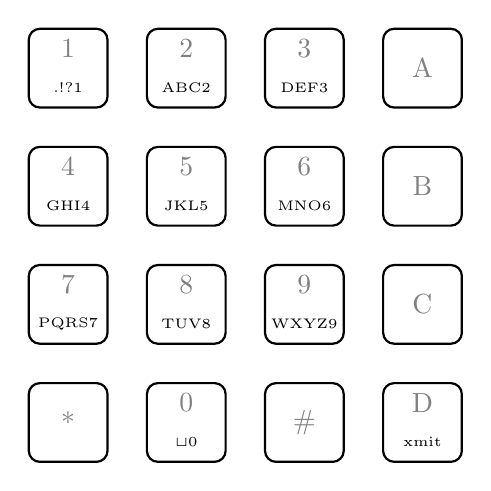
\begin{tikzpicture}[x=1mm, y=1mm]
            \draw[rounded corners=4, thick] (0,45) rectangle (10,55) ++(-5,-2.5) node {\textcolor{gray}{1}} ++(0,-5) node {\tiny .!?1};
            \draw[rounded corners=4, thick] (15,45) rectangle (25,55) ++(-5,-2.5) node {\textcolor{gray}{2}} ++(0,-5) node {\tiny ABC2};
            \draw[rounded corners=4, thick] (30,45) rectangle (40,55) ++(-5,-2.5) node {\textcolor{gray}{3}} ++(0,-5) node {\tiny DEF3};
            \draw[rounded corners=4, thick] (45,45) rectangle (55,55) node[pos=.5] {\textcolor{gray}{A}};
            \draw[rounded corners=4, thick] (0,30) rectangle (10,40) ++(-5,-2.5) node {\textcolor{gray}{4}} ++(0,-5) node {\tiny GHI4};
            \draw[rounded corners=4, thick] (15,30) rectangle (25,40) ++(-5,-2.5) node {\textcolor{gray}{5}} ++(0,-5) node {\tiny JKL5};
            \draw[rounded corners=4, thick] (30,30) rectangle (40,40) ++(-5,-2.5) node {\textcolor{gray}{6}} ++(0,-5) node {\tiny MNO6};
            \draw[rounded corners=4, thick] (45,30) rectangle (55,40) node[pos=.5] {\textcolor{gray}{B}};
            \draw[rounded corners=4, thick] (0,15) rectangle (10,25) ++(-5,-2.5) node {\textcolor{gray}{7}} ++(0,-5) node {\tiny PQRS7};
            \draw[rounded corners=4, thick] (15,15) rectangle (25,25) ++(-5,-2.5) node {\textcolor{gray}{8}} ++(0,-5) node {\tiny TUV8};
            \draw[rounded corners=4, thick] (30,15) rectangle (40,25) ++(-5,-2.5) node {\textcolor{gray}{9}} ++(0,-5) node {\tiny WXYZ9};
            \draw[rounded corners=4, thick] (45,15) rectangle (55,25) node[pos=.5] {\textcolor{gray}{C}};
            \draw[rounded corners=4, thick] (0,0) rectangle (10,10) node[pos=.5] {\textcolor{gray}{*}};
            \draw[rounded corners=4, thick] (15,0) rectangle (25,10) ++(-5,-2.5) node {\textcolor{gray}{0}} ++(0,-5) node {\tiny $\sqcup$0};
            \draw[rounded corners=4, thick] (30,0) rectangle (40,10) node[pos=.5] {\textcolor{gray}{\#}};
            \draw[rounded corners=4, thick] (45,0) rectangle (55,10) ++(-5,-2.5) node {\textcolor{gray}{D}} ++(0,-5) node {\tiny xmit};
        \end{tikzpicture}
        \caption{Mapping of Keypad Keys to Characters} \label{fig:keypad}
    \end{figure}
    \item \textit{Fixing a character:} \label{spec:finalizeCharacter} There are three ways to make a character a permanent part of the message and to advance the cursor:
        \begin{enumerate}
            \item If the user presses a different key than the one they've been using to create a character, then the cursor will advance, and the system shall start a new character creation sequence in accordance with Requirement~\ref{spec:createCharacter}.
            \item If the user presses the \textbf{right pushbutton}, then the cursor will advance (unless doing so violates Requirement~\ref{spec:boundCursor}), but the system will not start a new character sequence until the user presses a key.
            \item If 2~seconds have passed since the user last pressed a key or pushbutton, then the cursor will advance (unless doing so violates Requirement~\ref{spec:boundCursor}), but the system will not start a new character sequence until the user presses a key.
        \end{enumerate}
    \item \textit{Deleting a character:} \label{spec:deleteCharacter} The \textbf{left pushbutton} shall be used to delete a character.
        \begin{enumerate}
            \item If the cursor is under a character being created, then the cursor will remain in position, and the character being created shall be cleared until the user presses a key.
            \item If the cursor is under a blank space at the end of a non-empty message, then the cursor will move back one position, and the character that is now above the cursor shall be cleared.
        \end{enumerate}
    \item \textit{The cursor is bound to the message:} \label{spec:boundCursor} If the cursor is under a blank space at the end of the message, then pressing the right pushbutton shall have no effect.
        If the cursor is under a blank space at the start of the message, then pressing the left pushbutton shall have no effect.
        If the cursor is under a blank space at the end of the message, then the cursor will not advance in response to the passage of time.
    \item \textit{Press indicator:} \label{spec:pressIndicator} Whenever the user presses a key, the \textbf{right LED} shall illuminate for approximately \textonequarter second.\footnote{
            In Section~\ref{subsec:blinking}, we will approximate \textonequarter second as 256ms.
        }
    \item \textit{Transmitting the message:} \label{spec:transmission} If the user presses the \texttt{D} key on the \textbf{numeric keypad}, then:
        \begin{enumerate}
            \item the message shall be printed on the Serial Monitor, and immediately thereafter
            \item the message shall be cleared from the editor, and the system shall be readied to construct a new message.
        \end{enumerate}
\end{enumerate}